% Options for packages loaded elsewhere
\PassOptionsToPackage{unicode}{hyperref}
\PassOptionsToPackage{hyphens}{url}
%
\documentclass[
]{article}
\usepackage{amsmath,amssymb}
\usepackage{lmodern}
\usepackage{iftex}
\ifPDFTeX
  \usepackage[T1]{fontenc}
  \usepackage[utf8]{inputenc}
  \usepackage{textcomp} % provide euro and other symbols
\else % if luatex or xetex
  \usepackage{unicode-math}
  \defaultfontfeatures{Scale=MatchLowercase}
  \defaultfontfeatures[\rmfamily]{Ligatures=TeX,Scale=1}
\fi
% Use upquote if available, for straight quotes in verbatim environments
\IfFileExists{upquote.sty}{\usepackage{upquote}}{}
\IfFileExists{microtype.sty}{% use microtype if available
  \usepackage[]{microtype}
  \UseMicrotypeSet[protrusion]{basicmath} % disable protrusion for tt fonts
}{}
\makeatletter
\@ifundefined{KOMAClassName}{% if non-KOMA class
  \IfFileExists{parskip.sty}{%
    \usepackage{parskip}
  }{% else
    \setlength{\parindent}{0pt}
    \setlength{\parskip}{6pt plus 2pt minus 1pt}}
}{% if KOMA class
  \KOMAoptions{parskip=half}}
\makeatother
\usepackage{xcolor}
\usepackage[margin=1in]{geometry}
\usepackage{graphicx}
\makeatletter
\def\maxwidth{\ifdim\Gin@nat@width>\linewidth\linewidth\else\Gin@nat@width\fi}
\def\maxheight{\ifdim\Gin@nat@height>\textheight\textheight\else\Gin@nat@height\fi}
\makeatother
% Scale images if necessary, so that they will not overflow the page
% margins by default, and it is still possible to overwrite the defaults
% using explicit options in \includegraphics[width, height, ...]{}
\setkeys{Gin}{width=\maxwidth,height=\maxheight,keepaspectratio}
% Set default figure placement to htbp
\makeatletter
\def\fps@figure{htbp}
\makeatother
\setlength{\emergencystretch}{3em} % prevent overfull lines
\providecommand{\tightlist}{%
  \setlength{\itemsep}{0pt}\setlength{\parskip}{0pt}}
\setcounter{secnumdepth}{-\maxdimen} % remove section numbering
\ifLuaTeX
  \usepackage{selnolig}  % disable illegal ligatures
\fi
\IfFileExists{bookmark.sty}{\usepackage{bookmark}}{\usepackage{hyperref}}
\IfFileExists{xurl.sty}{\usepackage{xurl}}{} % add URL line breaks if available
\urlstyle{same} % disable monospaced font for URLs
\hypersetup{
  pdftitle={Causal Inference Report: Review on Child Penalties Across Countries: Evidence and Explanations},
  pdfauthor={Juan Pablo Brasdefer; Fabian Pawelczyk},
  hidelinks,
  pdfcreator={LaTeX via pandoc}}

\title{Causal Inference Report: Review on Child Penalties Across
Countries: Evidence and Explanations}
\author{Juan Pablo Brasdefer \and Fabian Pawelczyk}
\date{2023-05-24}

\begin{document}
\maketitle

\begin{verbatim}
## 
## Attaching package: 'ggdag'
\end{verbatim}

\begin{verbatim}
## The following object is masked from 'package:stats':
## 
##     filter
\end{verbatim}

\hypertarget{abstract}{%
\section{Abstract}\label{abstract}}

According to the DAG shown in Figure @ref(fig:dag\_plot), there is a
causal relationship between the variable ``birth\_having\_child'' and
``earnings.'' @ref(tab:dag\_plot) @ref(fig:dag\_plot)

The paper we analyzed examines the influence of having children on the
gross labor earnings of both mothers and fathers (the estimand).
Specifically, it delves into the \emph{child penalty} - a phenomenon
referring to the potential decrease in earnings experienced by
individuals, particularly women, upon becoming parents. This `penalty'
essentially represents the earnings disparity between those with
children and those without.

The authors aim to contribute to the extensive literature on gender
inequality by applying an \emph{event study methodology}, with the birth
of the first child serving as the central event. Utilizing a rich panel
dataset that provides information on labor market outcomes and children,
the authors navigate through the complex dynamics of parenthood and
earnings, aiming to shed light on how gender inequality in earnings
might be perpetuated by the advent of parenthood.

\hypertarget{dag-and-extension}{%
\section{DAG and extension}\label{dag-and-extension}}

We present the baseline DAG in Figure X where the estimand is shown in
the most simplest way. However, the authors admit that earning penalties
can come from three margins, nameley: the extensive margin of labor
supply (employment), the intensive margin of labor supply (hours worked)
and finally the wage rate (denoted by \emph{w}). We include this into a
new DAG (Figure X) to make clear that that the earnings consist of
different parts. @ref(fig:dag\_plot).

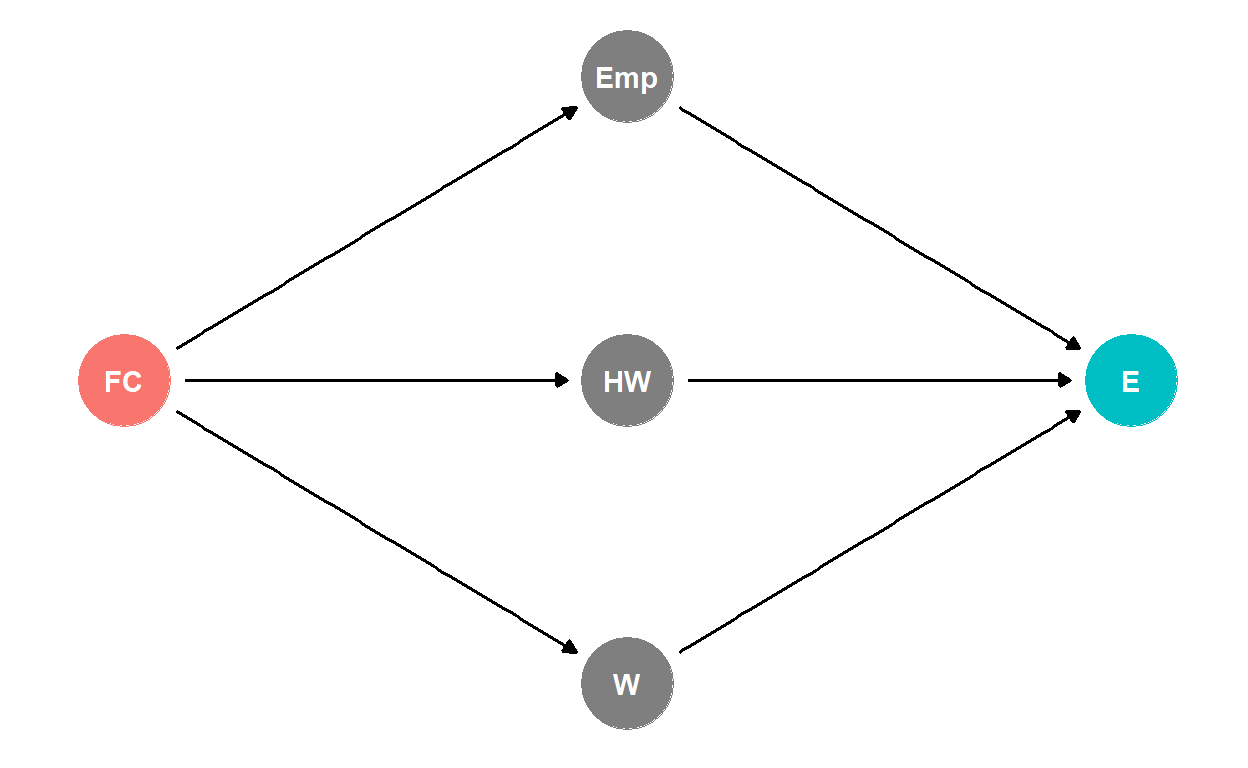
\includegraphics{ci-brasdefer-pawelczyk-report-new_files/figure-latex/unnamed-chunk-2-1.pdf}
Now let me use \ref{fig:figs}

\begin{figure}
\centering
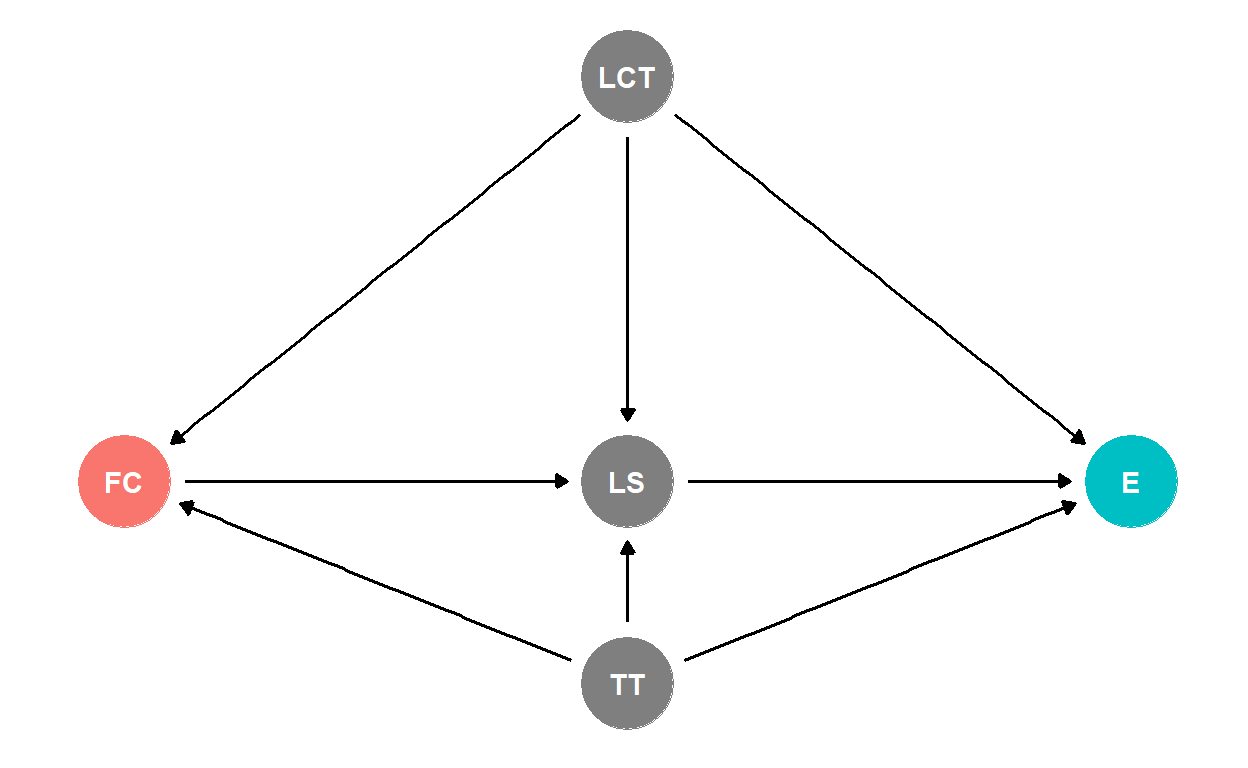
\includegraphics{ci-brasdefer-pawelczyk-report-new_files/figure-latex/unnamed-chunk-3-1.pdf}
\caption{Directed Acyclic Graph (DAG) showing the hypothesized
relationships between having a First Child (FC), Employment (Emp), Hours
Worked (HW), Wage (W), and Earnings (E). This model is a simplification,
and the effects of additional children and other potential confounding
factors are also captured in the analysis.}
\end{figure}

\begin{figure}
\centering
\includegraphics{ci-brasdefer-pawelczyk-report-new_files/figure-latex/unnamed-chunk-4-1.pdf}
\caption{Directed Acyclic Graph (DAG) showing the hypothesized
relationships between having a First Child (FC), Labor Supply (LS),
Life-Cycle Trends (LCT), Time Trends (TT), and Earnings (E). LS
represents the combined effect of employment status, hours worked, and
wage. LCT and TT are confounders that are controlled for in the
analysis. This model is a simplification, and the effects of additional
children are also captured in the analysis.}
\end{figure}

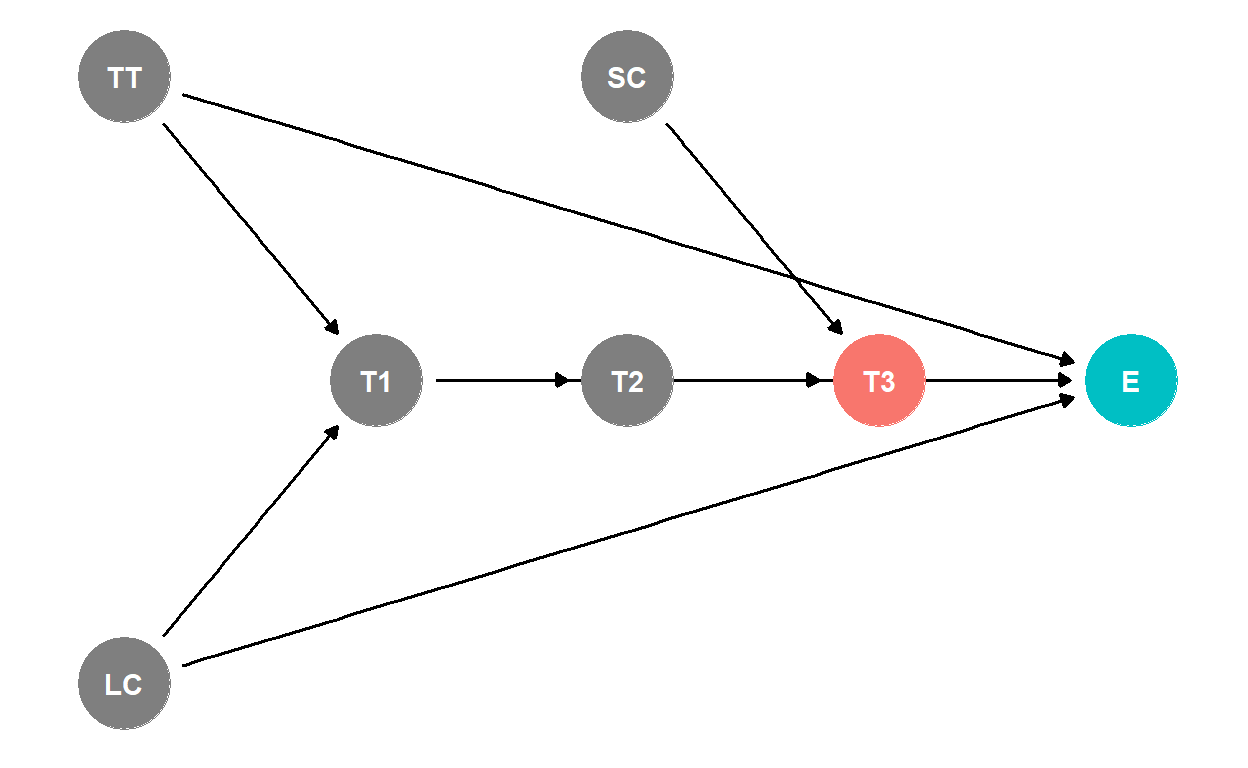
\includegraphics{ci-brasdefer-pawelczyk-report-new_files/figure-latex/unnamed-chunk-5-1.pdf}

@ref(fig:dag\_plot)

\begin{figure}

{\centering 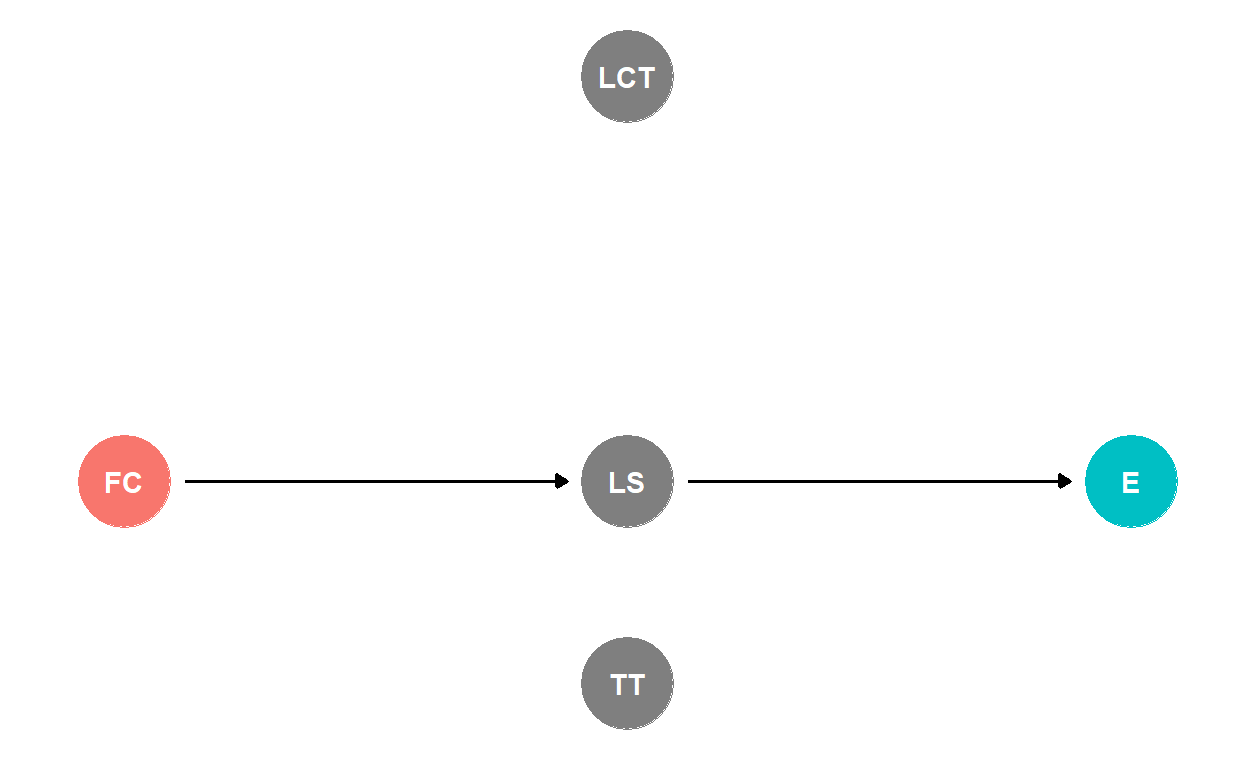
\includegraphics[width=1\linewidth]{ci-brasdefer-pawelczyk-report-new_files/figure-latex/dag5-1} 

}

\caption{This is DAG 5}\label{fig:dag5}
\end{figure}

\hypertarget{walk-through-the-causal-inference-pipeline}{%
\section{Walk through the causal inference
pipeline}\label{walk-through-the-causal-inference-pipeline}}

\hypertarget{first-what-is-the-estimand}{%
\section{First, what is the
estimand?}\label{first-what-is-the-estimand}}

The estimand: Impact of children on the earnings of women relative to
men. Then let's ref this shit \texttt{\textbackslash{}ref(fig:dag5)}

\[Y^{g}_{\text{ist}} = \sum_{j \neq -1} \alpha^{g}_{j} \cdot I[j = t] + \sum_k \beta^{g}_{k} \cdot I[k = \text{age}_{is}] + \sum_y \gamma^{g}_{y} \cdot I[y = s] + \nu^{g}_{\text{ist}}
\]

\hypertarget{advanced-identification-strategy-did-and-iv-variables}{%
\section{Advanced identification strategy: DID and IV
variables}\label{advanced-identification-strategy-did-and-iv-variables}}

\hypertarget{instrumental-variable-event-study}{%
\subsection{Instrumental Variable Event
Study}\label{instrumental-variable-event-study}}

To validate whether the authors identification strategy is valid the
authors run two main identification checks in order to test the
robustness of the results and therefore to address potential bias and
establish a causal inference.

In this identification check, the authors propose a variation of their
event study approach by introducing an Instrumental Variable (IV)
strategy. They use the gender composition of the first two children as
an instrument for having a third child, following the reasoning that
parents with two same-sex children are more likely to have a third
child. The validity of this instrument relies on the assumption that the
sex of the first two children doesn't independently impact labor market
outcomes (the exclusion restriction).

The authors modify their event study specification to estimate the Local
Average Treatment Effect (LATE) of having a third child in order to
compare it with the IV approach. This means they are focusing on the
subpopulation influenced by the instrument (the ``compliers''). For the
interested reader we created a DAG to visualize this IV approach (see
Figure X).

To facilitate a valid comparison, the authors modify their event study
model as follows:

\[Y^{}_{\text{istt'}} = \sum_{j \neq -1} \alpha^{}_{j} \cdot I[j = t] + \sum_k \beta^{}_{k} \cdot I[k = \text{age}_{is}] + \sum_y \gamma^{}_{y} \cdot I[y = s] + \sum_{n \neq -1} \delta^{}_{n} \cdot I[j = t'] + \nu^{}_{\text{istt'}}
\]

In this model, t' represents the event time with respect to the third
child. The new term \(∑ δ_n · I[n = t']\) introduces event time dummies
for the birth of the third child. The authors also keep the event time
dummies for the first child, as previous childbearing dynamics may
impact the effect of the third child.

The IV specification is identical, except it includes an additional
instrumenting strategy which instruments the event time dummies around
the third child birth using the sex mix of the first two children:

\[I[n = t'] = I[n = t'] * I[same sex siblings]\]

In other words, \(I[n = t']\) takes the value of one when the woman is
at event time t' with respect to the third child and her first two
children are of the same sex.

Following the logic from the baseline model the counterfactual outcome,
denoted \(\tilde{Y}^w_{istt'}\), is calculated excluding the effect of
the third child but including the effects of the first child and other
controls. It represents the expected labour market outcome for a woman
if she did not have a third child, providing a baseline against which to
compare the actual outcomes of those who did have a third child.

The findings suggest that the event study and IV estimates align
closely, indicating robustness in their empirical approach. The
short-run effect of the third child is similar to that of the first,
showing an earnings reduction of 20-30\%. However, the long-run effect
of a third child is about 5\%, lower than the long-run effect of the
first child for those who only have one child, suggesting a diminishing
marginal effect with the addition of more children.

\begin{figure}

{\centering \includegraphics[width=1\linewidth]{ci-brasdefer-pawelczyk-report-new_files/figure-latex/unnamed-chunk-7-1} 

}

\caption{Note: This DAG represents a way to think about the aforementioned IV approach. T3 denotes the timing of the third child that is instrumentalized through the sex composition (SC). Also, to get rid of the confunders LC and TT the authors are controlling for it. E - Earnings, T1 - First Child, T2 - Second Child, T3 - Third Child, SC - Sex Composition, TT - Time Trends, LC - Life Cycle Trends}\label{fig:unnamed-chunk-7}
\end{figure}

\hypertarget{critics}{%
\section{Critics}\label{critics}}

While the authors are able to identify a causal effect and have a rather
strong methodological foundation there are still some things one can
discuss.

\hypertarget{comparision-among-countries-and-different-sources-of-earnings}{%
\subsection{Comparision among countries and different sources of
earnings}\label{comparision-among-countries-and-different-sources-of-earnings}}

One critic that do not purely roots in the measurement itself but comes
into play when comparing the measurements among countries are different
parntel leave benefits. Since the earnings measure choosen by the
authors also include any (non-mandated) parental leave benefits it could
be that cross-country comparision reflect the variation of, for
instance, parental leave benfit policies. We therefore extend the DAG
from the beginning and add a new stream that consist \texttt{earnings}
in the model. Note that we simplify here. It is also likely that
parental leave benefits have direct effects on the decision to bear
children, since it reduces financial stress on parenthood. Controlling
for the amount of those benefits is advisable.
\includegraphics{ci-brasdefer-pawelczyk-report-new_files/figure-latex/unnamed-chunk-8-1.pdf}

\hypertarget{causal-effect-vs-causal-mechanism}{%
\subsection{Causal Effect vs Causal
Mechanism}\label{causal-effect-vs-causal-mechanism}}

While the authors deliver rather strong evidence on the existence of a
causal effect the underlying mechanism is still unclear. The name child
\emph{penalty} suggests a punishment espically towards mothers but what
if mothers decide to take jobs with more flexibility in order to raise
their children? Maybe, economically speaking this increases their
utility instead of punishes them. To understand the mechanism better it
would be good to extend the research here and see in what kind of
branches women move after bearing children. Is it a more family-friendly
sector or is it the wage-rate that decreases even though women stay in
the same sector.

One explaination for the differences in the penalties could have to do
with government policies. While numerous studies have been conducted to
evaluate the influence of public policies, such as taxes, transfers, and
family-focused policies like parental leave and child care provisions,
on gender gaps and female labor supply, these policies do not adequately
explain the ``child penalties'' experienced by mothers in the workforce.

Another pontentially fruitful approach to explain this phenomen is to
take a deeper look into gender-norms in given societies. Thi\ldots{}

\hypertarget{authors-do-not-control-for-having-only-one-child}{%
\subsection{Authors do not control for having only one
child}\label{authors-do-not-control-for-having-only-one-child}}

The author's analysis does not control for those parents that only have
one child. As a result, the long-term child penalties that we observe
include the impacts of having additional children, and therefore, are
influences by total fertility. To overcome this short-term we would
suggest to run an additional model with a \texttt{only-one-child}
variable.

\end{document}
